\section{Солнечная активность и её изменения со временем}

Внешняя структура Солнца от внутренних к внешним:

\begin{itemize}
	\item Фотосфера – видимый диск. На определенном радиусе на определенной длине полны Солнце перестает быть прозрачным (оптическая толщина примерно равна 1).
	
	\item Хромосфера – цветной ореол вокруг Солнцы, его «внутренняя атмосфера».
	
	\item Корона --- часть внешней атмосферы Солнца, очень разреженная и протяжённая часть.
\end{itemize}

Основной механизм охлаждения фотосферы --- это излучение, а основным механизмом ее нагрева служат поднимающиеся из недр Солнца мелкомасштабные конвективные потоки (более крупные конвективные ячейки, ответственные за появление крупномасштабной хромосферной сетки, находятся глубже). Выход конвективных потоков наблюдается как мелкомасштабная ячеистая структура фотосферы, образуемая непрерывно возникающими и исчезающими областями повышенной яркости — гранулами — с довольно резкими границами. Характерный размер гранул \~ 1500 км., а время их существования --- 5-10 минут. Скорости конвективных потоков не превышают нескольких км/с. Газ поднимается, остывает и опускается вниз между ячейками за новой порцией энергии. В отдельных областях фотосферы, как правило, вблизи солнечных пятен, наблюдаются протяженные области повышенной яркости, образуемые цепочками многочисленных более «горячих» гранул. Это \textbf{факелы}, или \textbf{факельные поля} — долгоживущие образования (могут существовать месяцами), связанные с более интенсивным конвекционным переносом тепла из нижележащих слоев Солнца. Напряженность магнитного поля в факелах составляет несколько сотен Гауссов — недостаточно для того чтобы затормозить конвекцию. Температура газа в факелах на несколько сотен К выше окружающей поверхности. 

Самыми заметными деталями фотосферы являются солнечные пятна. \textbf{Солнечные пятна} – области активности. Пятна тёмные, так как там ниже температура (примерно на 1500К). Подвод тепла к ним осуществляется снизу, но в области пятен подвод тепла подавляется сильным магнитным полем. 

Пятна связаны с Солнечной активностью. Пятен больше, когда Солнце активнее. Нет, Солнце не светит слабее в это время, ведь за энерговыделение отвечают термоядерные реакции внутри (а пятна обусловлены процессами во внешних слоях звезды)

\subsection{Про подавление конвекции под пятнами}

Каждое пятно — это место выхода в атмосферу из недр Солнц а трубки силовых линий магнитного поля. Поскольку эти линии замкнутые, они образуют широкую петлю над фотосферой. Обычно пятна образуются парами в местах входа и выхода силовых линий поля петли (биполярная структура). Если средняя индукция поля в фотосфере Солнца порядка 1 Гаусса, то в пятнах она составляет от нескольких сотен до нескольких тысяч Гауссов. Плотность энергии поля при этом достаточно велика, чтобы в силу вмороженности поля в газ затормозить конвекцию, препятствуя движению газа по замкнутым линиям тока. Резкое уменьшение притока энергии из недр Солнца и является причиной локального падения температуры и образования пятна. Энергия, не достигшая фотосферы в области пятен, частично выходит на поверхность благодаря усиленной конвекции в факелах. Группы пятен вместе с окружающими их факелами называют активными областями на Солнце. Силовые линии магнитных полей, связанных с активными областями, могут уходить высоко в верхние слои солнечной атмосферы, где они подчиняют себе движение сильно разреженного ионизованного газа. Поэтому над активной областью структура магнитного поля, как и поле скоростей газа, и его плотность, оказываются крайне неоднородными.

И солнечные вспышки, и корональные выбросы — это результат преобразования энергии магнитного поля в другие формы энергии, вызванного развитием плазменных неустойчивостей в магнитном поле со сложной конфигурацией силовых линий. Частота появления таких событий меняется как из месяца в месяц, так и из года в год — в такт изменению общей активности Солнца. 

\textbf{Солнечные вспышки.} Это ещё одно проявление активности Солнца. В результате пересоединения линий магнитного поля выделяется энергия. Полное энерговыделение не очень большое, но энергия выделяется быстро.

Если вспышка сопровождается выбросом плазмы (около $10^{15}$ г) – \textbf{корональные выбросы}. Выброшенная плазма может взаимодействовать с атмосферой земли, долетая до неё за 1-4 дня.

Солнечные вспышки наблюдать трудно. Их обнаруживают из-за увеличения потока УФ и радиоизлучения. Однако были и визуальные наблюдения астрономами-любителями, кроме того, есть данные по геомагнитному шторму. Так, в длинных проводниках могут наводится большие токи, увеличивается активность полярных сияний.

Солнечные вспышки — лишь наиболее яркое проявление активных процессов на Солнце. Под активностью Солнца понимают целый комплекс явлений в различных слоях его атмосферы, обусловленных выходом магнитных полей в активных областях. Над активными областями атмосфера Солнце по всей ее толщине имеет более высокую плотность и температуру, и поэтому обладает более высокой яркостью в коротковолновом диапазоне. Горячий газ образует многочисленные петли самых различных размеров, отражающие структуру силовых линий магнитного поля. Эти петли отчетливо наблюдаются в мягких рентгеновских лучах. Подъем активности Солнца проявляется в более частом образовании как активных областей фотосферы, так и очень горячих очагов в короне над центрами активности, более частом образовании солнечных вспышек и корональных выбросов.

\subsection{Цикл солнечной активности (Швабе, 1843)} 

Этот цикл связан с изменением глобального магнитного поля Солнца. Глобальное магнитное поле Солнца \~ 1 Гаусс. За 11 лет меняется полярность поля, оно переворачивается. (То есть совсем честный полный цикл 22 года). 

Активность Солнца подвержена изменениям с периодом, лежащим в пределах 8–13 (в среднем 11) лет. Есть указания на существование колебаний активности с более короткими и с более длинными периодами, но они выражены не столь явно, как 11-летний цикл. Рост очередного цикла активности начался в конце 2009 г. В годы минимума на Солнце может в течение долгого времени не наблюдаться никаких пятен или вспышек, а в годы максимума иногда одновременно существуют десятки пятен, образующие отдельные группы. Далекое УФ и рентгеновское излучение Солнца как звезды также подвержено резким колебаниям, отражающим уровень солнечной активности. Меняется с циклом активности и общий вид короны, отражающий конфигурацию крупномасштабного магнитного поля. В минимуме активности структура поля более простая, близкая к дипольной, и корона вытянута вдоль экватора. Вблизи максимума она становится более сферически симметричной. Корональные лучи, наблюдаемые в любой фазе цикла, дают начало «спокойному» солнечному ветру, интенсивность которого также подвержена изменениям и связана с уровнем активности Солнца.

Таким образом, активность Солнца претерпевает некоторую эволюцию, которая плохо описана. Наблюдалось несколько минимумов активности, самый известный из которых – маундеровский (см. рисунок \ref{fig:7_sunspot}).

\begin{figure}[H]
	\centering
	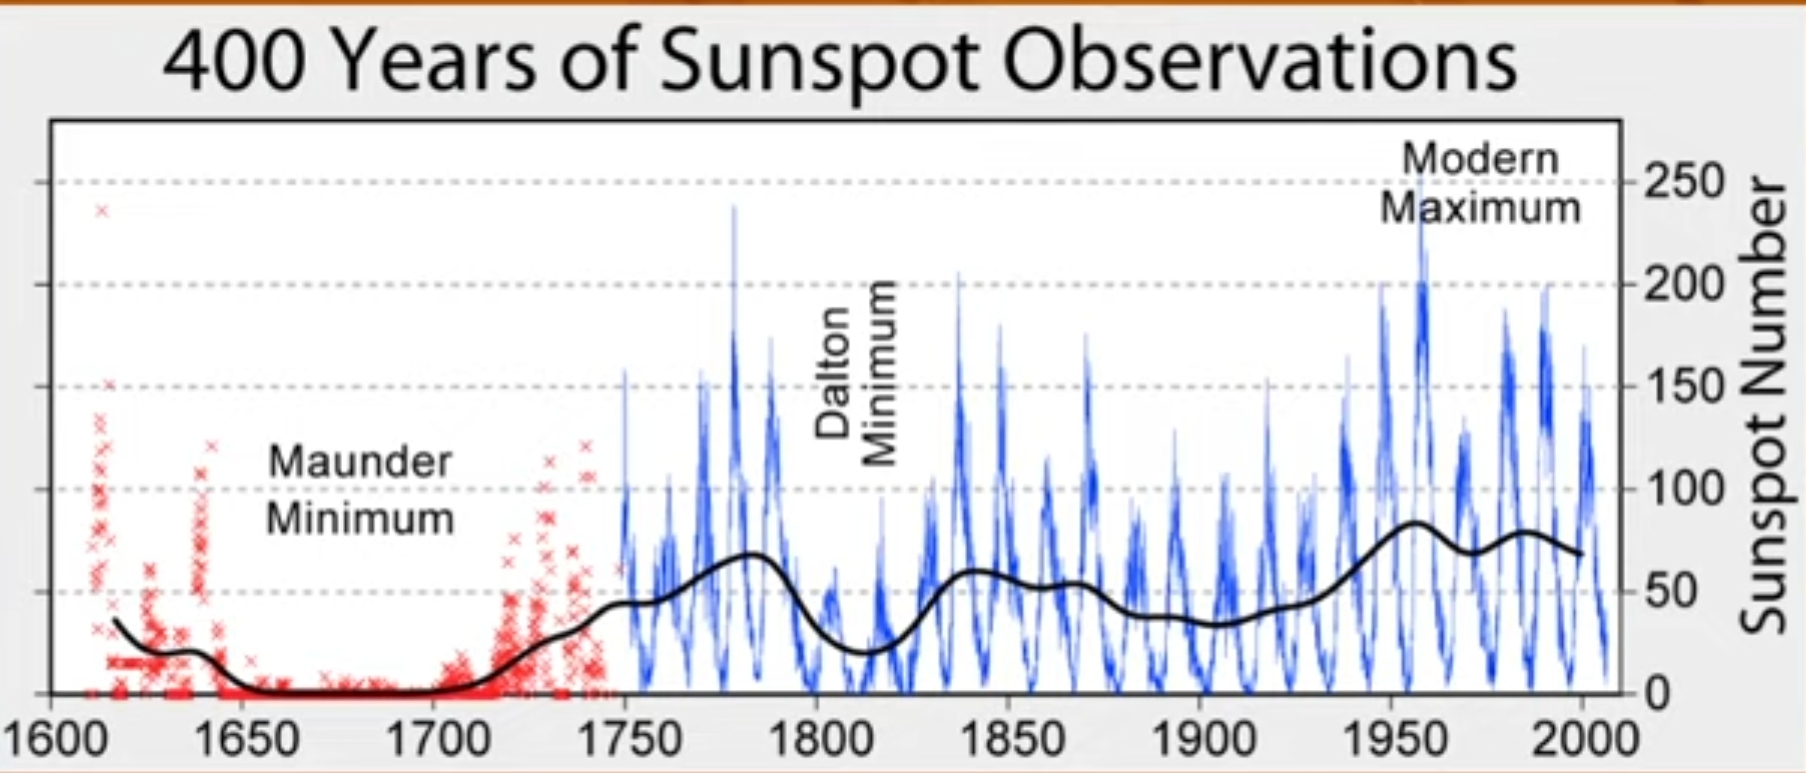
\includegraphics[width=0.7\linewidth]{7_sunspot}
	\caption{Солнечная активность от года}
	\label{fig:7_sunspot}
\end{figure} 

Мощные солнечные вспышки и корональные выбросы влияют на физические условия в космическом пространстве, в магнитосфере и ионосфере Земли, ее радиационных поясах. Высокая радиация может вывести из строя электронную космическую аппаратуру или представлять опасность для космонавтов. Наибольшее влияние солнечной активности испытывают внешние, ионизованные слои земной атмосферы. Но опосредованно активность Солнца сказывается и на поверхности Земли, на многих явлениях живой и неживой природы — от роста нестабильности атмосферной циркуляции до увеличения частоты сердечно-сосудистых кризов. Отдельные звенья сложных цепочек, обуславливающих связь земных явлений с активностью Солнца, пока плохо изучены. Уровень активности Солнца отслеживается и прогнозируется в ряде стран специальными службами Солнца.

\subsection{Реконструкция солнечной активности на большом масштабе времени}

Учёные пытаются восстановить солнечную активность на временах порядка тысяч лет. Это делается с помощью анализа содержания космогенных изотопов. Эти изотопы образуются в верхней атмосфере Земли под действием галактических космических лучей. То есть это частицы высоких энергий, которые прилетают в нашу систему откуда-то. Внутри гелиосферы доминирует солнечный ветер, то есть поток от Солнца мешает космическим лучам проникать внутрь Солнечной системы. Поэтому, когда активность Солнца выше, поток галактических космических лучей на уровне верхней атмосферы Земли меньше. Это приводит к тому, что образуется меньше, например, бериллия-10 и углерода-14. Поэтому, анализируя относительную долю этих изотопов в различных образцах, если мы умеем датировать эти образцы, можно делать выводы об активности Солнца. Например, можно анализировать ледяные керны и годичные кольца деревьев и говорить что-то об активности Солнца в далёком прошлом. Удаётся получить точность в несколько десятилетий.

\textbf{Глобальная эволюция Солнца}. Эта эволюция происходит на масштабе миллиарда лет, она никак не связана с описанными выше ~ 50ти летними минимумами и максимумами.
